\documentclass{article}
\usepackage[letterpaper]{geometry}
\geometry{verbose,tmargin=1in,bmargin=1in,lmargin=1in,rmargin=1in}

\usepackage[utf8]{inputenc}
\usepackage{amsmath}
\usepackage{listings}
\usepackage{graphicx}
\usepackage{enumitem}
\usepackage{amssymb}
\usepackage{tabularx}
\usepackage{hyperref}
\usepackage{caption}
\usepackage{float}
\usepackage[section]{placeins}
\usepackage{empheq}
\usepackage{stackengine}
\usepackage{subcaption}
\usepackage{array}
\usepackage[super]{nth}

\def\delequal{\mathrel{\ensurestackMath{\stackon[1pt]{=}{\scriptstyle\Delta}}}}


\title{CIS 680: Project 1 Part B}
\author{Junfan Pan}
\date{09/19/2020}

\begin{document}
    \maketitle
    
    \section{Adversarial Images}
    \noindent
    \begin{enumerate}
    	\item[1.1] 
    	Untargeted Attack with pre-trained neural network\\
        \begin{figure}[H]
     	\centering
     	\begin{subfigure}[b]{0.45\textwidth}
         	\centering
         	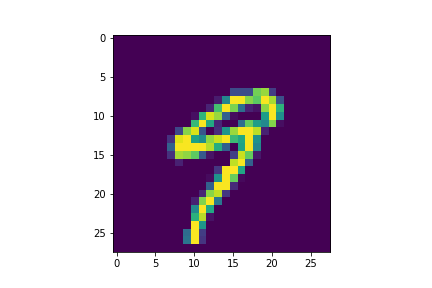
\includegraphics[width=\textwidth]
         	{image/No.0 original test_image.png}
         	\caption{original image}
         	\label{fig:Hyperplane Epoch 0}
     	\end{subfigure}
     	\hfill
     	\begin{subfigure}[b]{0.45\textwidth}
         	\centering
         	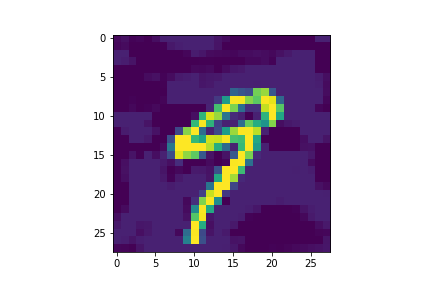
\includegraphics[width=\textwidth]
         	{image/No.0 perturbed test_image.png}
         	\caption{untargeted attack image}
         	\label{fig:Hyperplane Epoch 1000}
     	\end{subfigure}
     	\end{figure}
     	
     	\begin{figure}[H]
     	\centering
     	\begin{subfigure}[b]{0.45\textwidth}
         	\centering
         	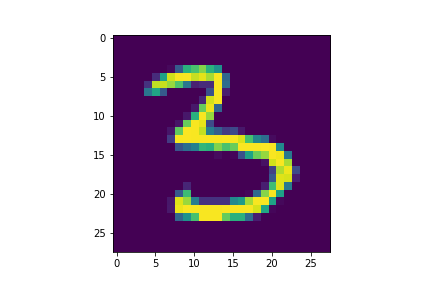
\includegraphics[width=\textwidth]
         	{image/No.1 original test_image.png}
         	\caption{original image}
         	\label{fig:Hyperplane Epoch 0}
     	\end{subfigure}
     	\hfill
     	\begin{subfigure}[b]{0.45\textwidth}
         	\centering
         	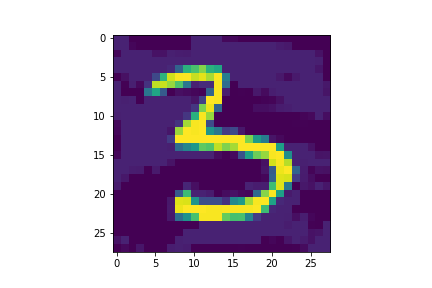
\includegraphics[width=\textwidth]
         	{image/No.1 perturbed test_image.png}
         	\caption{untargeted attack image}
         	\label{fig:Hyperplane Epoch 1000}
     	\end{subfigure}
     	\end{figure}
     	\begin{itemize}
     	\item
     	Describe the difference between adversarial images and original images\\
     	In the adversarial images, some pixels around the digits become lighter which let the network to misclassify as different digits.
        \end{itemize}
        
        \item[1.2] 
    	Targeted Attack with pre-trained neural network\\
     	\begin{figure}[H]
     	\centering
     	\begin{subfigure}[b]{0.45\textwidth}
         	\centering
         	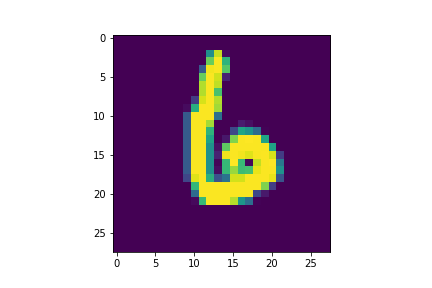
\includegraphics[width=\textwidth]
         	{image/No.2 original test_image.png}
         	\caption{original image}
         	\label{fig:Hyperplane Epoch 0}
     	\end{subfigure}
     	\hfill
     	\begin{subfigure}[b]{0.45\textwidth}
         	\centering
         	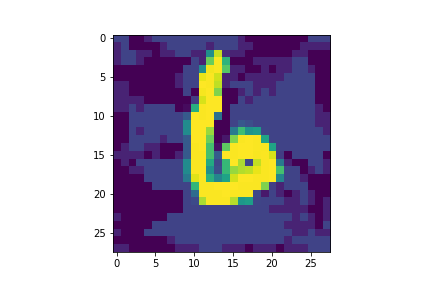
\includegraphics[width=\textwidth]
         	{image/No.2 perturbed test_image.png}
         	\caption{targeted attack image with target value as 4}
         	\label{fig:Hyperplane Epoch 1000}
     	\end{subfigure}
     	\end{figure}
     	\begin{itemize}
     	\item
     	In the adversarial images with targeted attack, more pixels around the digits in the whole image become lighter comparing with those adversarial images generated by untargeted attack.
        \end{itemize}
        
        \item[1.3] 
        
    	Targeted and Untargeted Attack using pre-trained neural network and re-trained neural network\\
	    \begin{minipage}[t]{\linewidth}
    	\captionsetup{type=figure}
        \centering
        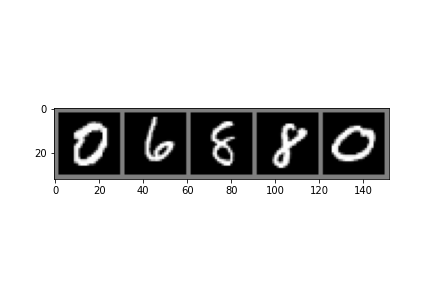
\includegraphics[width=0.65\linewidth]{image/pre_batch_untarget_original_image.png}
        \caption{original image with all correct prediction as 0,6,8,8,0} 
        \label{original image with all correct prediction as 0,6,8,8,0}     
        \end{minipage}
        
     	\begin{figure}[H]
     	\centering
     	\begin{subfigure}[b]{0.45\textwidth}
         	\centering
         	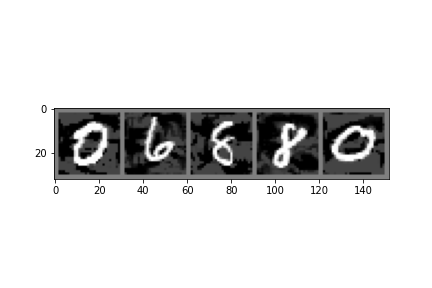
\includegraphics[width=\textwidth]
         	{image/pre_batch_untarget_new_image.png}
         	\caption{untargeted attack image using pre-trained network with prediction as 2, 2, 6, 4, 2}
         	\label{fig:Hyperplane Epoch 0}
     	\end{subfigure}
     	\hfill
     	\begin{subfigure}[b]{0.45\textwidth}
         	\centering
         	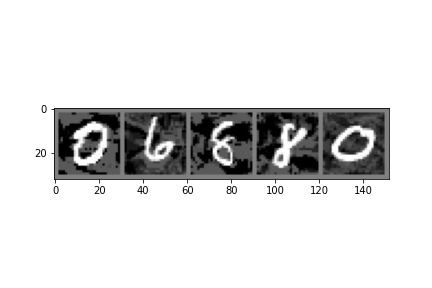
\includegraphics[width=\textwidth]
         	{image/pre_batch_target_new_image.png}
         	\caption{targeted attack image using pre-trained network with target value 2, 4, 6, 4, 4}
         	\label{fig:Hyperplane Epoch 1000}
     	\end{subfigure}
     	\end{figure}
     	
     	\begin{figure}[H]
     	\centering
     	\begin{subfigure}[b]{0.45\textwidth}
         	\centering
         	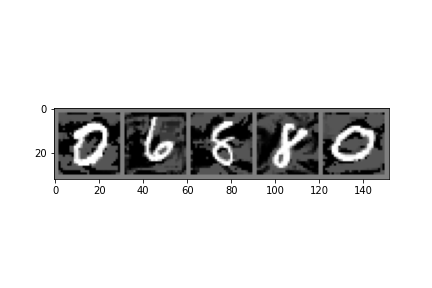
\includegraphics[width=\textwidth]
         	{image/re_batch_untarget_new_image.png}
         	\caption{untargeted attack image using re-trained network with prediction as 2, 3, 6, 6, 9}
         	\label{fig:Hyperplane Epoch 0}
     	\end{subfigure}
     	\hfill
     	\begin{subfigure}[b]{0.45\textwidth}
         	\centering
         	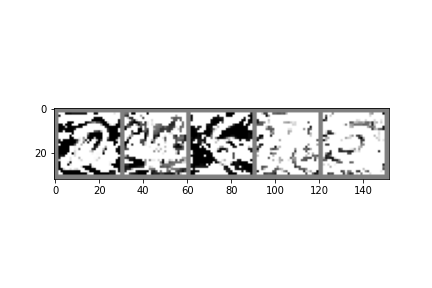
\includegraphics[width=\textwidth]
         	{image/re_batch_target_new_image.png}
         	\caption{targeted attack image using re-trained network with target value as 2, 4, 6, 4, 4}
         	\label{fig:Hyperplane Epoch 1000}
     	\end{subfigure}
     	\end{figure}
     	
        \begin{itemize}
    	\item
    	Comparing the adversarial images generated by untargeted attack and targeted attack, we can see that it is easier to achieve the former one.\\
    	
    	\item
        Networks trained using the same structures with same training datasets but with different initializations, the adversarial images generated from the same test examples can still be different. In addition, if we want to use the targeted attack with the same target value, it is possible that the previous network can easily achieve it while for the re-trained network it can be very difficult. We can observe that the adversarial images generated using targeted attack with re-trained network are almost all blurred and we almost can't see anything.

    \end{itemize}
    \end{enumerate}
    
        
\end{document}  